% ---------------------------------------------------------------------------
% Body of the article; built into article.pdf by `make` (see Makefile).
% Structure follows published ReScience C replications: replication summary
% first, then analysis of the original paper, set-up, implementation, results.
% ---------------------------------------------------------------------------

\section{Introduction}

\citet{Moulds:2015} presented lulcc, an R package for spatially explicit land use
change modelling, with an explicit aim: to make land use change models open, so that
their results can be reproduced and their code examined and extended. They
demonstrated the package on the Plum Island Ecosystems data set, which ships with
it, going through the stages of an inductive model: suitability from logistic
regression, demand from interpolation between observed maps, spatial allocation by
CLUE-S \supercite{Verburg:2002} and by an ordered procedure \supercite{Fuchs:2013},
and pattern validation by three-map comparison \supercite{Pontius:2011}.

We replicate that application in Python: a replication in the sense of
\citet{NASEM:2019}, with new code and our own runs, rather than a reproduction with the
original code. Both lulcc and the CLUE-S implementation we use were written from the
published description of the algorithm \supercite{Verburg:2002}, independently of each
other. Ours comes from LuccME \supercite{Aguiar:2012}, a land use change framework
developed at INPE on the TerraME modelling platform \supercite{Carneiro:2013}, which
organises a model into demand, potential and allocation components and has supported
land use and emission scenarios for the Brazilian Amazon \supercite{Aguiar:2016} and
for Brazil \supercite{Bezerra:2022}. The original article itself lists LuccME among
the implementations of CLUE-S. Allocation procedures are known to leave room for
different readings, with consequences for the simulated maps \supercite{Mazy:2023};
the comparison therefore tests two independent readings of the same description, with
lulcc's own demonstration as the reference.

\section{Replication summary}

Figure~\ref{fig:method} summarises the replication. On the left is the reference: lulcc
1.0.4 running the article's own demonstration script, in a Docker image. On the right is
the replication, which runs on DisSModel \supercite{DisSModel:2026}, a Python framework
for spatially explicit dynamic models, and its land use package DisSLUCC
\supercite{DisSLUCC:2026}. In the centre are the four stages of the original model
(Section~\ref{sec:model}), each implemented separately on both sides. The code of the
replication is original, and its parts have three origins, shown in the right-hand boxes:
\begin{itemize}
  \item \emph{CLUE-S allocation}: the component of DisSLUCC 0.5.0, used unchanged at
    the deterministic level. It was ported, before and independently of this work, from
    the discrete allocation of LuccME, \texttt{AllocationD\-ClueS\-Like}, and not from
    lulcc. In the three LuccME test labs that use it, DisSLUCC 0.5.0 reproduces the
    outputs of TerraME with the same number of iterations in every year and differences
    of at most $1.2 \times 10^{-7}$ \supercite{DisSLUCCbenchmark:2026}.
  \item \emph{Written for this replication, without reference to lulcc's code}: reading
    the data, the logistic regression (statsmodels) and its AUC, and the potential that
    passes suitability and elasticity to the CLUE-S allocation.
  \item \emph{Ports of lulcc's code}: the demand rounding, the stratified training sample,
    the random perturbation of CLUE-S (a subclass of the DisSLUCC component that replaces
    its iteration loop), the ordered allocation, and the three-map comparison with its
    agreement budget and figure of merit. They follow the original article, and where it
    leaves a choice open they follow lulcc's procedure step by step, in Python
    (Section~\ref{sec:analysis}); their agreement with lulcc verifies the ports, not an
    independent reading.
\end{itemize}

\begin{figure}[t]
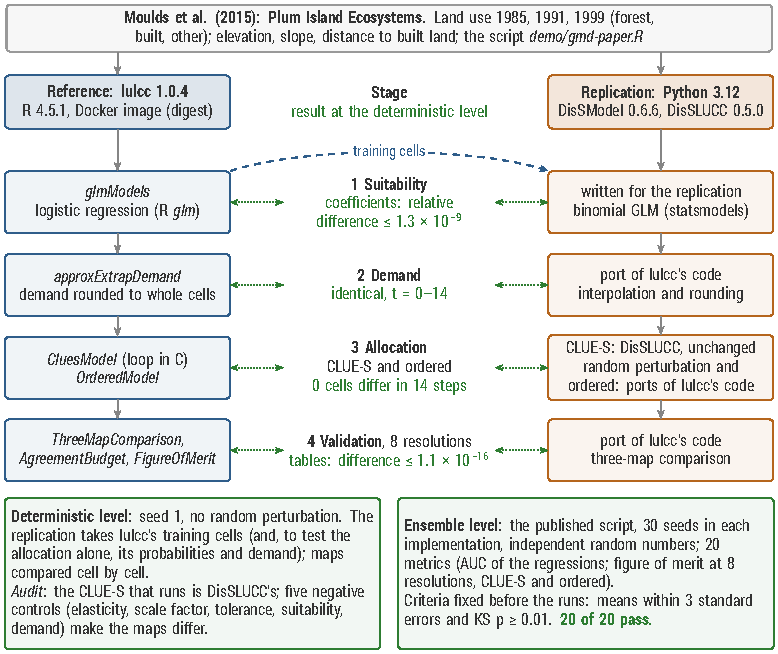
\includegraphics[width=\linewidth]{figures/fig_method.pdf}
\caption{The replication and its comparison with lulcc. Left: the reference, lulcc's
functions in the demonstration script. Right: the replication and the origin of each
part. Centre: the four stages of the original model and, in green, the result of the
deterministic comparison at each stage (Table~\ref{tab:deterministic}). The dashed arrow
is the only input that the replication's own chain takes from the reference. Bottom:
the two levels of comparison (Section~\ref{sec:comparison}).}
\label{fig:method}
\end{figure}

The comparison has two levels, at the bottom of Fig.~\ref{fig:method}. At the
\emph{deterministic} level the randomness is removed from both sides, and the stages can be
fed with the reference's own inputs, so that a difference points at one stage; run as a
whole chain, the replication takes from lulcc only the cells of the training sample,
because R's random sample cannot be drawn again in Python. At the \emph{ensemble} level
both sides run the published script, with its randomness, using independent random
numbers, and are compared in distribution.

Three parts of the original application are not replicated: the regression trees and
random forests of the paper's Fig.~5, since we did not reimplement R's rpart and
randomForest; the agreement budget at the ensemble level, which is compared only at the
deterministic level; and the published curves of Figs.~7--8, whose values the paper does
not give.

Given the same inputs, the CLUE-S allocation of DisSLUCC reproduces every simulated map
of lulcc cell by cell, and so do our ports of the ordered allocation and of the
validation tables (to $10^{-16}$). With
independent random numbers, 30 runs of each implementation agree in distribution on all
20 metrics compared, under criteria recorded before the runs. Running the original
demonstration script required one repair, unrelated to the model
(Section~\ref{sec:obstacles}).

\section{The original model}
\label{sec:model}

The Plum Island Ecosystems data set\supercite{Pontius:2014} covers a site in north-east
Massachusetts on a grid of $434 \times 497$ cells of about 100\,m (99.92\,m by
99.95\,m), 113\,563 of them inside the study area. It holds land use maps for 1985,
1991 and 1999 (forest, built, other), treated as time points 0, 6 and 14, and three
explanatory variables: elevation, slope and distance to built land in 1985.

\paragraph{Suitability.} One binary logistic regression per class is fitted on a
stratified random sample of 10\% of the cells of the 1985 map: built on the three
variables, forest and other on elevation and slope. The paper also fits regression
trees and random forests and compares the three model types by the area under the
ROC curve (AUC) on the remaining cells (its Fig.~5), and evaluates the glm for built
on the cells that became built between 1985 and 1991 (its Fig.~6).

\paragraph{Demand.} The number of cells of each class at every time point from 0 to
14 is interpolated linearly between the three observed maps and rounded to integers
that sum to the number of cells.

\paragraph{CLUE-S allocation.} At each time step every cell receives, for each class,
its suitability plus an elasticity (0.2 for all classes) if the cell already belongs to
that class. Each cell is allocated to the class with the highest value plus a
class-specific iteration term; the term is then increased by the difference between
demand and allocated area, times a scale factor ($10^{-6}$), until the largest
difference is at most 50 cells. At every iteration the suitability is perturbed by a
uniform random number in $[-0.0002, 0.0002]$ (\texttt{jitter.f}).

\paragraph{Ordered allocation.} Classes are visited in a fixed order (built, forest,
other). A class with rising demand takes the most suitable cells not yet settled; a
class with falling demand releases its least suitable cells. In the stochastic
version a cell qualifies only if its suitability exceeds (or, when releasing, falls
below) a uniform random number.

\paragraph{Validation.} The initial observed map (1985), the final observed map (1999)
and the simulated map for 1999 are compared at eight resolutions, aggregating
$2 \times 2$ to $256 \times 256$ cells, through the three-dimensional contingency table
of \citet{Pontius:2011}. The paper reports the agreement budget and the figure of merit
of the forest-to-built transition for both allocation methods (its Figs.~7 and 8).

\section{Analysis of the original paper}
\label{sec:analysis}

The article states the model, its parameters and the code that produced its figures,
which the package ships as a demonstration script (\texttt{demo/gmd-paper.R}). Four
aspects are nonetheless not determined by the text.

\paragraph{Random numbers without a seed.} Three steps draw random numbers: the training
sample, the CLUE-S perturbation and the stochastic ordered allocation. The script sets
no seed, so the numbers printed in the paper are one draw from a distribution and
cannot be repeated exactly, not even with lulcc. This is why we generated the
reference ourselves and compare at two levels (Section~\ref{sec:comparison}).

\paragraph{Choices left to the code.} The text describes the following steps at the
level of the algorithm. We followed lulcc's source code for them, so that a difference
in the comparison would point at the algorithm rather than at a convention:
\begin{itemize}
  \item demand rounding: rows rescaled to the number of cells, floored, and the
    remaining cells given to the classes with the largest remainders. LuccME rounds
    differently, adding each year's increment to the previous year's rounded demand, so
    this is a convention on which the two implementations differ;
  \item training sample: the class codes are numeric, so the stratification of
    \texttt{caret::}\allowbreak\texttt{createDataPartition}, which lulcc calls, groups
    them by quantile, which for this map gives two strata, \{forest, built\} and
    \{other\};
  \item ordered allocation: which cells are candidates, the temporary class for
    released cells, the limit of 1000 random draws, and ties kept in cell order;
  \item three-map comparison: the layout of the table, aggregation blocks anchored at
    the upper-left corner with incomplete edge blocks weighted by their number of
    valid cells, and empty denominators left out of the sums.
\end{itemize}
The CLUE-S allocation of DisSLUCC was not modified to match lulcc.

\paragraph{Behaviours visible only in the code.} The random forest models receive a
numeric 0/1 response and therefore run in regression mode. The CLUE-S loop has a second
stopping condition based on the mean signed difference between demand and allocation;
because the rounded demand sums to the number of cells, that mean is zero, and only the
largest difference stops the iteration.

\paragraph{Iterations not reported.} lulcc does not report the number of iterations of
CLUE-S at each step, so only the map produced at each step can be compared, not the path
of the iteration. Against LuccME the iteration counts are compared and agree.

\paragraph{Results shown only as figures.} The AUCs are printed in the figures, but the
agreement budgets and figures of merit are only drawn (Figs.~7--8). We compare the
latter with our own runs of lulcc, not with the published curves.

\section{Computational set-up}
\label{sec:setup}

\paragraph{Data.} The replication reads the Plum Island Ecosystems data set from GeoTIFF
files exported from the R package (\texttt{data(pie)}), without any other change; the
exported layers carry the original CRS (NAD83, Massachusetts Mainland, EPSG:26986).

\paragraph{Reference.} We ran the demonstration script with lulcc 1.0.4
\supercite{lulcc:2019} and archived the outputs \supercite{lulccgoldens:2026}. Two
references were produced:
\begin{itemize}
  \item a \emph{deterministic} one, with the randomness removed (seed 1 for the
    training sample, \texttt{jitter.f} $= 0$, ordered allocation not stochastic),
    exported stage by stage: training cells, regression coefficients, the suitability
    matrix, the demand table, all simulated maps and the three-map tables, with doubles
    written to 17 significant digits;
  \item an \emph{ensemble} of 30 runs of the script as published, seeds 1 to 30.
\end{itemize}
The only change to the script is the repair described in
Section~\ref{sec:obstacles}.

\paragraph{Software.} Reference: a Docker image based on rocker/geospatial 4.5.1 (pinned by digest,
\texttt{sha256:6483198da9a6\ldots}; full digest in the goldens' \texttt{Dockerfile}), with
R 4.5.1 and packages from a dated snapshot of CRAN (1 October 2026): lulcc 1.0.4, raster
3.6-32, sp 2.2-0, caret 7.0-1, ROCR 1.0-12, randomForest 4.7-1.2, rpart 4.1.27. The lulcc
1.0.4 on CRAN was republished in November 2025, but its source package is the one built
by the author in February 2019. Replication: Python 3.12, DisSModel 0.6.6, DisSLUCC 0.5.0,
NumPy 2.5, SciPy 1.18, statsmodels 0.15, rasterio 1.5.

\paragraph{Hardware and time.} The reference and the replication were run on one
desktop computer (Dell OptiPlex 7050, Intel Core i7-7700T at 2.9\,GHz, Ubuntu). One run of CLUE-S over the 14 steps took
on average 11\,s in lulcc, whose inner loop is in C, and about 20\,s in the
replication; the ordered allocation took 3\,s and 0.2\,s. One complete run of the
paper's experiment, including the regression trees and random forests of lulcc, took
about 90\,s in R; one run of the replication, about 30\,s.

\section{Implementation}

Suitability is fitted with statsmodels (binomial GLM). The AUC is computed by the
Mann--Whitney statistic, with ties counted as one half. CLUE-S is the allocation
component of DisSLUCC (\texttt{AllocationDClue\-SLike}) on a DisSModel raster backend;
the simulation starts at time 1, as lulcc does, and the suitability with elasticity is
supplied to it in double precision. The random perturbation is added by a subclass of
the DisSLUCC component that replaces its iteration loop and draws a new uniform number
for every cell and class at every iteration; a test in the repository checks that, with
the perturbation set to zero, it gives the same result as the published component. The ordered allocation and the three-map comparison are separate
modules, operating on the valid cells in the raster's row-major order, which is also
lulcc's cell order.

\paragraph{Why the maps can be identical.} Two independently written implementations of
an iterative allocation give the same map only if they agree on everything that decides
a cell. lulcc's C loop and DisSLUCC's component do. The score of a class in a cell is its
suitability, plus the elasticity if the cell belonged to that class at the start of the
step, plus a class term that starts at zero at every step. Each cell takes the class with
the highest score, the first class in order on a tie. After each pass the class term
grows by the difference between demand and allocated cells times the scale factor, and
the loop stops when the largest absolute difference is at most the tolerance (lulcc's
second condition, on the mean difference, is inactive; Section~\ref{sec:analysis}). The
parameters of DisSLUCC were translated from lulcc's, not tuned: the scale factor as
\texttt{factor\_iteration}, the tolerance as \texttt{max\_difference}, a cell area of 1 so
that demand is counted in cells, and a transition matrix of ones, the rule matrix of the
demonstration script. The two differ only where this application never goes: at the
iteration limit DisSLUCC stops with an error, lulcc returns the last map with a warning.

\section{Comparison and acceptance criteria}
\label{sec:comparison}

Criteria were recorded in the code repository before either ensemble was run; the
commit that adds them precedes those with results.

\paragraph{Deterministic level.} Each stage is fed with the reference's own inputs, so
that a difference points at that stage only (centre of Fig.~\ref{fig:method}). Coefficients and suitability must agree
within numerical precision; demand, allocated maps and validation tables must be
identical or agree to rounding error.

\paragraph{Ensemble level.} Our 30 runs (seeds 1 to 30 of NumPy's default generator) are
compared with lulcc's 30 on 20 metrics: the AUC of the glm for each class and for the
gain of built, and the figure of merit of forest to built for each allocation method at
each of the eight resolutions. A metric passes if the means differ by at most three
standard errors of the difference and a two-sample Kolmogorov--Smirnov test gives
$p \geq 0.01$. The regression trees and random forests of the paper's Fig.~5 are
outside the criteria: we did not reimplement R's rpart and randomForest, and other
implementations would differ by construction.

\section{Results}

\subsection{Deterministic level}
\label{sec:det}

Table~\ref{tab:deterministic} lists the stages; the main results are also shown in the centre
of Fig.~\ref{fig:method}. The CLUE-S allocation of DisSLUCC,
given lulcc's suitability and demand, produced the same map as lulcc at each of the
14 time steps, cell by cell; it needed 51 iterations at the first step and 257 at the
last. The ordered allocation also matched at every step, and the three-map tables and
figures of merit agreed to rounding error. Running the whole chain from our own
regression gave the same final map: the coefficients differ by about $10^{-9}$ in
relative terms, which did not change any allocation. The same holds when the suitability
is computed by DisSLUCC's own logistic potential, in single precision, from lulcc's
coefficients, so the whole chain of DisSLUCC reproduces lulcc.

The agreement is not an artefact of the comparison. The CLUE-S that runs is the
component of the installed package, called once per step; from the reference only the
suitability and the demand are read, never a simulated map; lulcc's map changes at every
step (12\,733 cells at the first, 440 to 590 at the others), and ours matches the same
step and not the neighbouring ones. The comparison also fails when it should: changing
one thing at a time makes the final maps differ, by 4\,555 cells for an elasticity of
0.25 instead of 0.2, 130 for a demand shifted by 100 cells, 45 for a tolerance of 10
cells instead of 50, 14 for noise of $10^{-4}$ added to the suitability and 6 for a
scale factor doubled. These checks are in \texttt{scripts/audit.py}.

\begin{table}[h]
\footnotesize
\begin{tabular}{p{0.5\linewidth}p{0.42\linewidth}}
\toprule
Stage & Result \\
\midrule
Observed transitions 1985--1999 (paper, Sect.~3.2) & identical \\
Regression coefficients, same training cells & max.\ relative difference $1.3 \times 10^{-9}$ \\
Suitability from lulcc's coefficients & max.\ difference $9 \times 10^{-14}$ \\
Suitability from our coefficients & max.\ difference $2.8 \times 10^{-10}$ \\
Demand, $t = 0, \dots, 14$ & identical \\
CLUE-S, 14 steps & 0 cells differ at every step \\
Ordered allocation, 14 steps & 0 cells differ at every step \\
Three-map tables, 8 resolutions, both methods & max.\ difference $1.1 \times 10^{-16}$ \\
Figure of merit forest $\to$ built & max.\ difference $2.2 \times 10^{-16}$ \\
Whole chain from our own regression & final map identical \\
DisSLUCC's own logistic potential (single precision) & 0 cells differ at every step \\
Perturbation subclass with perturbation 0 & 0 cells differ at every step \\
\bottomrule
\end{tabular}
\caption{Deterministic level: each stage fed with the reference's inputs.}
\label{tab:deterministic}
\end{table}

Figure~\ref{fig:maps} shows the observed maps and the 1999 maps simulated by CLUE-S in
both implementations, which the original article does not show: it reports the
simulations only through the agreement budget and the figure of merit. The
replication's map comes from its whole chain, with its own regression and demand; only
the training cells are taken from the reference. The two simulated maps are the same
map. Both look more clustered than the observed 1999 map, an
impression we did not quantify; since the two maps are identical, it is a property of the
model and its set-up, not of either implementation.

\begin{figure}[h]
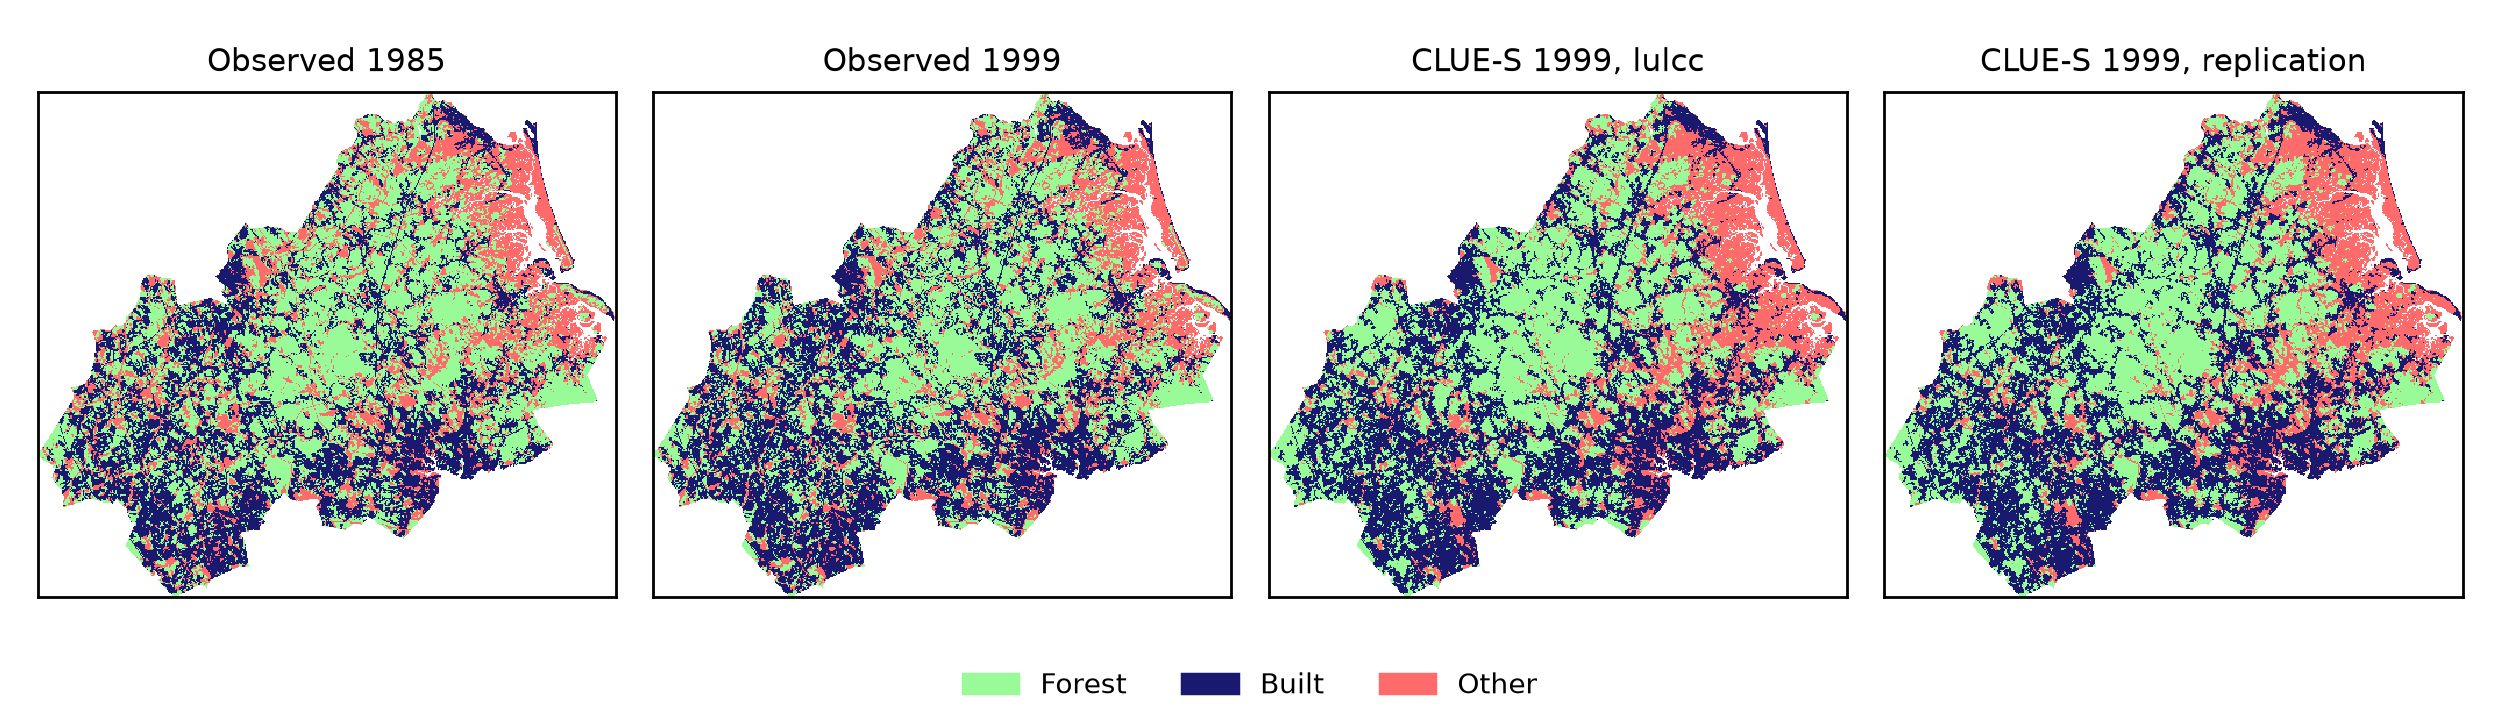
\includegraphics[width=\linewidth]{figures/fig_maps.png}
\caption{Land use observed in 1985 and 1999, and simulated for 1999 by CLUE-S without
perturbation, by lulcc and by the replication (its own regression, demand and DisSLUCC's
allocation; training cells of the reference). 0 cells differ between the two simulated
maps. Colours as in Fig.~3 of the original article.}
\label{fig:maps}
\end{figure}

\subsection{Ensemble level}

All 20 metrics passed. Table~\ref{tab:ensemble} shows a selection and
Figure~\ref{fig:fom} the figure of merit at every resolution; the spread between runs
is the same in both implementations, including the larger spread of the stochastic
ordered allocation.

The criteria detect a wrong model but not every wrong detail. With an elasticity of
0.25, ten runs of the replication fail seven of the eight figure-of-merit metrics of
CLUE-S; without any perturbation they fail none. Most of the spread between runs comes
from the training sample, and the perturbation changes only a few cells (19 in the
final map of one run), so the ensemble level confirms the distribution of the results,
not the implementation of the perturbation.

\begin{table}[h]
\footnotesize
\setlength{\tabcolsep}{4pt}
\begin{tabular}{lccccc}
\toprule
Metric & lulcc & replication & diff. & tol. & KS $p$ \\
 & mean (sd) & mean (sd) & & & \\
\midrule
AUC glm, forest & 0.6439 (0.0007) & 0.6437 (0.0006) & $-0.0003$ & 0.0005 & 0.07 \\
AUC glm, built & 0.9382 (0.0003) & 0.9382 (0.0003) & $-0.0001$ & 0.0002 & 0.81 \\
AUC glm, other & 0.7295 (0.0010) & 0.7290 (0.0008) & $-0.0004$ & 0.0007 & 0.14 \\
AUC glm, gain of built & 0.6446 (0.0004) & 0.6446 (0.0004) & $0.0000$ & 0.0003 & 0.81 \\
FoM CLUE-S, factor 2 & 0.1168 (0.0017) & 0.1167 (0.0019) & $-0.0001$ & 0.0014 & 0.81 \\
FoM CLUE-S, factor 16 & 0.3766 (0.0058) & 0.3756 (0.0062) & $-0.0010$ & 0.0046 & 0.81 \\
FoM CLUE-S, factor 256 & 0.7684 (0.0052) & 0.7688 (0.0052) & $+0.0004$ & 0.0040 & 0.96 \\
FoM ordered, factor 2 & 0.1079 (0.0017) & 0.1079 (0.0019) & $0.0000$ & 0.0014 & 1.00 \\
FoM ordered, factor 16 & 0.4311 (0.0188) & 0.4308 (0.0199) & $-0.0003$ & 0.0150 & 0.96 \\
FoM ordered, factor 256 & 0.6795 (0.0326) & 0.6784 (0.0327) & $-0.0011$ & 0.0253 & 1.00 \\
\bottomrule
\end{tabular}
\caption{Ensemble level, 30 runs each (selection of the 20 metrics; all passed).
FoM: figure of merit of the forest-to-built transition at 1999. Tolerance: three
standard errors of the difference of means. Differences are computed before
rounding.}
\label{tab:ensemble}
\end{table}

\begin{figure}[h]
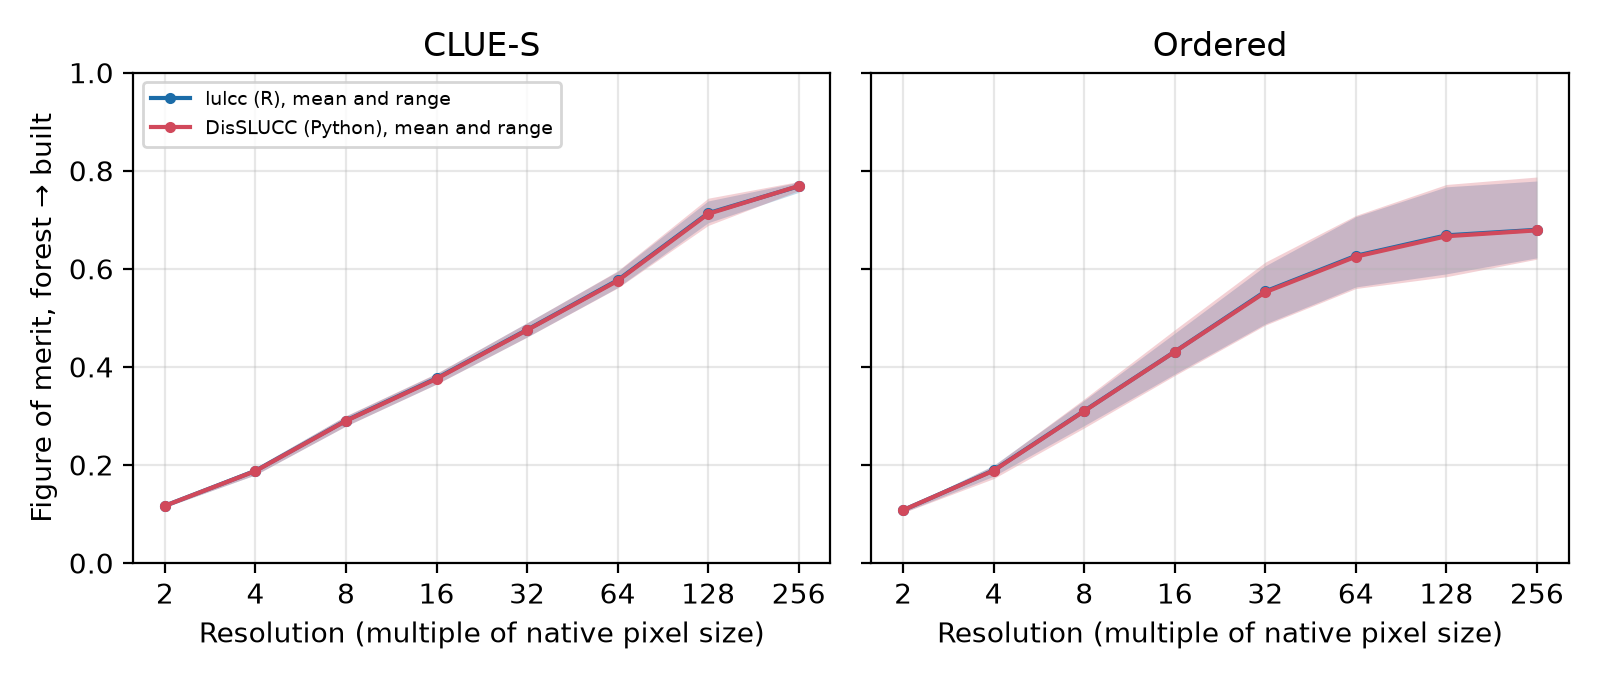
\includegraphics[width=\linewidth]{figures/fig_fom_forest_built.png}
\caption{Figure of merit of the forest-to-built transition against resolution, as in
Fig.~8 of the original article: mean and range of 30 runs of lulcc and of the
replication.}
\label{fig:fom}
\end{figure}

\subsection{The published values}

The values printed in the paper fall inside lulcc's own spread with one exception. In
our 30 runs of lulcc, the paper's AUC for built (0.9384) is at the 70th percentile,
that for the gain of built (0.6448) at the 63rd and that for other (0.7276) at the
7th; the AUC for forest (0.6423) is slightly below the lowest of the 30 runs (0.6425).
The paper used lulcc 1.0 with the R of 2015; our reference used lulcc 1.0.4 on current
R. We did not investigate the difference further. It is not unexpected: a value from the
same distribution falls outside the range of 30 runs with probability 2/31, about 6\%,
and for at least one of four AUCs with probability about 23\%.

\section{Obstacles}
\label{sec:obstacles}

\paragraph{The demonstration script does not run unchanged.} With current versions of
the raster and sp packages, the CLUE-S and ordered allocations stop with
\texttt{different crs}. The rasters of the data set were serialised by an old version
of raster, before the slot that holds the coordinate reference system in WKT form
existed; the allocation creates each simulated map from the initial one, the new
object carries a CRS in the current form and the old one does not, and the check that
precedes stacking them fails. Reassigning the CRS of the old objects does not help: it
leaves them with no CRS at all. Rebuilding each layer as a new raster object with the
same grid, values and CRS solves it; this is the only change we made to the script. A
package written to make land use models reproducible thus needed a repair to run
its own published example eleven years later, for a reason unrelated to the model.

\paragraph{An undeclared dependency.} lulcc loads the \texttt{gsubfn} package when it
builds the explanatory variables, but lists it only as a suggestion; it has to be
installed by hand.

\section{Conclusion}

The Plum Island Ecosystems application of lulcc was replicated. With the same inputs,
an independent implementation of CLUE-S reproduces lulcc's maps exactly, and so do our
ported ordered allocation and validation. That implementation was ported from LuccME
and reproduces LuccME's discrete labs, as a port should; what this replication adds is
that it also reproduces lulcc, so on this application the two independent readings of
the description of CLUE-S, in LuccME and in lulcc, coincide. With independent random numbers, the
two implementations agree in distribution on every metric compared. The main obstacle was
not in the model but in the environment around it.

\section*{Reproducing this replication}

Code: \url{https://github.com/LambdaGeo/rescience-lulcc}. Reference outputs and the
Docker environment that produces them: \url{https://github.com/LambdaGeo/lulcc-goldens}.
With the reference downloaded, \texttt{make env}, then \texttt{make check} (about one
minute), \texttt{make ensemble} (about 15 minutes) and \texttt{make compare} reproduce
Tables~\ref{tab:deterministic} and \ref{tab:ensemble} and Figure~\ref{fig:fom};
\texttt{make maps} draws Figure~\ref{fig:maps}, and \texttt{make audit} (about three
minutes) runs the checks of Section~\ref{sec:det}. Each takes the reference's directory
as \texttt{GOLDENS=}. The
versions of the Python packages are fixed in the file \texttt{requirements\allowbreak.lock}, and the R
environment of the reference in the Dockerfile of lulcc-goldens. The code is released
under GPL-3.0-or-later, the licence family of lulcc, because part of it follows lulcc's
source code.

\section*{Declaration of generative AI use}

A large language model from Anthropic (Claude Opus 5.5, in the claude.ai interface with
code execution) was used throughout this work, from the choice of the article to
replicate to this text, starting on 24 October 2026. It searched for and read the
original article and lulcc's source code; compared lulcc with DisSLUCC; wrote the
scripts that generate the reference outputs, the replication code and its tests, and
the comparison scripts; drafted the acceptance criteria; ran a first reference, the
deterministic comparison and both ensembles in a cloud workspace; found the cause of
the CRS error described in Section~\ref{sec:obstacles}; and drafted and typeset this
article. The decisions were the first author's: replicating this article, generating the
reference in a separate archive, using DisSLUCC unchanged and keeping the missing
pieces in the replication's repository, comparing at a deterministic and an ensemble
level, and keeping 30 runs. The CLUE-S implementation used, DisSLUCC, predates this
work. The first author regenerated the reference in the Docker image and reran the
comparison on his own computer, with the same results; the authors reviewed the code and
the text and are responsible for all the content. The tool is not listed as an author.
Commits made with it carry a Co-Authored-By line naming the model.

\section*{Acknowledgements}

We thank the developers of TerraME and LuccME at INPE, whose open code is the origin of
the CLUE-S implementation used here, and S. Moulds for making lulcc and its
demonstration openly available.

\noindent\emph{Complete table of the 20 ensemble metrics: see
\texttt{results/ensemble\_comparison.csv} in the code repository.}

